\documentclass[a4paper,14pt]{extarticle}

\usepackage{geometry}
\usepackage{amsmath,bm}
\usepackage{amssymb}
\usepackage{amsthm}
\usepackage{esint}
\usepackage{float}
\usepackage{graphicx}
\usepackage[dvipsnames]{xcolor}
\usepackage[utf8]{inputenc}
\usepackage[T2A]{fontenc}
%\usepackage[lutf8x]{luainputenc}

%\usepackage{fontspec}
%\setmainfont{CMU Serif}
%\setsansfont{CMU Sans Serif}
%\setmonofont{CMU Typewriter Text}

\usepackage[greek.polutoniko,english,russian]{babel}
% локализация и переносы
\usepackage{latexsym}
\usepackage{hhline}
\usepackage{multirow}
\usepackage{vmargin,indentfirst} 
\setmarginsrb{20mm}{15mm}{15mm}{15mm}{0mm}{0mm}{0mm}{10mm}
\usepackage[multiple]{footmisc}
\usepackage{hyperref}
\usepackage{multirow}
\usepackage{pdflscape}
%\numberwithin{equation}{section}
\usepackage[labelsep=period]{caption}


% команда для переноса строки внутри ячейки таблицы
\newcommand{\specialcell}[2][l]{%
  \begin{tabular}[#1]{@{}l@{}}#2\end{tabular}}

  \usepackage{physics}

\usepackage{tikz}
\usetikzlibrary{calc}
\usetikzlibrary{arrows.meta}

%\usepackage[margin=0.3in,bmargin=0.5in]{geometry}

%\usepackage{CJKutf8}%Chinese characters


\pagestyle{plain}

\theoremstyle{plain}
\newtheorem{theorem}{Theorem}[section]
\newtheorem{lemma}[theorem]{Lemma}
\newtheorem*{proposition}{Proposition}
\newtheorem{corollary}[theorem]{Corollary}
\newtheorem{problem}[theorem]{Problem}
\newtheorem{exercise}{Exercise}[section]

\theoremstyle{remark}
\newtheorem*{example}{Example}
\newtheorem*{examples}{Examples}
\newtheorem*{remark}{Remark}
\newtheorem*{hint}{Hint}

\theoremstyle{definition}
\newtheorem*{definition}{Definition}

\renewcommand{\emptyset}{\varnothing}
\newcommand\ph{\varphi}
\newcommand\eps{\varepsilon}

\newcommand\mbZ{\mathbb Z}
\newcommand\mbC{\mathbb C}
\newcommand\mbR{\mathbb R}
\newcommand\mbN{\mathbb N}
\newcommand\mbQ{\mathbb Q}
\newcommand\mbE{\mathbb E}

\newcommand\mcB{\mathcal B}
\newcommand\mcC{\mathcal C}
\newcommand\mcF{\mathcal F}
\newcommand\mcG{\mathcal G}
\newcommand\mcJ{\mathcal J}


\newcommand\la{\langle}
\newcommand\ra{\rangle}
\newcommand\ol{\overline}
\newcommand\ora{\overrightarrow}
\newcommand\rsa{\rightsquigarrow}

\DeclareMathOperator{\M}{M}
\DeclareMathOperator{\Span}{Span}
\DeclareMathOperator{\LL}{\cal L}
\DeclareMathOperator{\id}{id}
\DeclareMathOperator{\Ker}{Ker}
\DeclareMathOperator{\Img}{Im}
\DeclareMathOperator{\rk}{rank}
%\DeclareMathOperator{\Tr}{Tr}
\DeclareMathOperator{\cof}{cof}

\newcommand\dfn[1]{{\bf #1}}
\renewcommand{\thesubsubsection}{}

\newcounter{saveenumi}
\newcommand{\seti}{\setcounter{saveenumi}{\value{enumi}}}
\newcommand{\conti}{\setcounter{enumi}{\value{saveenumi}}}

\newcommand{\vct}[1]{\overrightarrow{#1}}
\newcommand{\bvct}[1]{\boldsymbol{#1}}
\newcommand{\codir}{\upuparrows}
\newcommand{\ncodir}{\uparrow \downarrow }

%% title background

\DeclareMathOperator{\sign}{sign}
\DeclareMathOperator{\const}{const}
\newcommand{\dprodd}[2]{\vct{#1}\cdot\vct{#2}}
\newcommand{\dprod}[2]{\bvct{#1}\cdot\bvct{#2}}

\newcommand{\cprod}[2]{\bvct{#1}\times\bvct{#2}}

\newcommand{\mprod}[3]{(\bvct{#1},\bvct{#2},\bvct{#3})}

\newcommand{\vecsys}{{$\bvct{a}_1$ , . . . , $\bvct{a}_n$ {}}}

\newcommand{\Problem}[1]{\vspace{\baselineskip}\textbf{Problem {#1}}\par}
\newcommand{\Solution}{\vspace{\baselineskip}\textbf{Solution}\par}

\newcommand*\coord[1]{%
  \begin{pmatrix}
    #1
  \end{pmatrix}%
}

\renewcommand{\d}[1]{\ensuremath{\operatorname{d}\!{#1}}}

\usepackage{tkz-euclide}
%\usetkzobj{all}

\usepackage{subcaption}

\usepackage{enumitem}

\usepackage{datetime}
\newdateformat{yeardate}{\THEYEAR}

\usepackage[toc,page]{appendix}

\def\contentsname{Содержание}

\usepackage{listings}

\lstset{% Собственно настройки вида листинга
inputencoding=utf8, extendedchars=\true, keepspaces = true, % поддержка кириллицы и пробелов в комментариях
language=C++,            % выбор языка для подсветки (здесь это Pascal)
basicstyle=\small\sffamily, % размер и начертание шрифта для подсветки кода
numbers=left,               % где поставить нумерацию строк (слева\справа)
numberstyle=\tiny,          % размер шрифта для номеров строк
stepnumber=1,               % размер шага между двумя номерами строк
numbersep=5pt,              % как далеко отстоят номера строк от подсвечиваемого кода
backgroundcolor=\color{white}, % цвет фона подсветки - используем \usepackage{color}
showspaces=false,           % показывать или нет пробелы специальными отступами
showstringspaces=false,     % показывать или нет пробелы в строках
showtabs=false,             % показывать или нет табуляцию в строках
frame=single,               % рисовать рамку вокруг кода
tabsize=2,                  % размер табуляции по умолчанию равен 2 пробелам
captionpos=t,               % позиция заголовка вверху [t] или внизу [b] 
breaklines=true,            % автоматически переносить строки (да\нет)
breakatwhitespace=false,    % переносить строки только если есть пробел
escapeinside={\%*}{*)}      % если нужно добавить комментарии в коде
}
\begin{document}



% Оформление титульного листа
\begin{titlepage}
\begin{center}
\textsc{Санкт-Петербургский государственный университет\\
Математико-механический факультет\\
Кафедра физической механики\\}

\vfill

\textsc{Методы измерений и электромеханические системы\\[3mm]}
Отчёт по лабораторной работе №2.2\\[6mm]


\textbf{\large<<Электронный осциллограф>>}

\vfill
\end{center}

\hfill
\begin{minipage}{.5\textwidth}
Выполнил студент:\\[2mm] 
Кручинина Екатерина Васильевна\\
группа: 24.Б51-мм\\[5mm]

Проверил:\\[2mm] 
к.ф.-м.н., доцент\\
Кац Виктор Михайлович
\end{minipage}%
\vfill
\begin{center}
 Санкт-Петербург, \yeardate\today\ г.
\end{center}
\end{titlepage}
% Содержание
\tableofcontents
\newpage
\section{Введение}

\subsection{Цель работы}
Целью данной лабораторной работы является исследование характеристик электронного осциллографа: измерение чувствительности пластин горизонтального и вертикального отклонения, максимальной чувствительности осциллографа, получение фигур Лиссажу и определение частоты исследуемого напряжения по фигурам Лиссажу, а также получение навыков обработки экспериментальных данных.

\subsection{Решаемые задачи}

В ходе выполнения работы решаются следующие задачи:


\begin{itemize}
\item Исследование чувствительности пластин вертикального и горизонтального
отклонений осциллографической трубки.
\item Наблюдение с помощью осциллографа синусоидального напряжения, полученного с
выхода генератора.
\item Получение фигуры Лиссажу и определение частоты исследуемого напряжения по
фигурам Лиссажу.
\end{itemize}

\newpage

\section{Основная часть}

\subsection{Теоретическая часть}
Осциллограф является одним из важнейших исследовательских приборов. Чаще всего он применяется для наблюдения и исследования переменных во времени электрических сигналов.

В состав осциллографа входят следующие основные элементы: электронно-лучевая трубка, система развертки, усилитель, синхронизатор. Основным рабочим элементом осциллографа является электронно-лучевая трубка. В ее состав входят электронная пушка и две пары взаимно перпендикулярных отклоняющих пластин: пластины вертикального отклонения (ПВО) и пластины горизонтального отклонения (ПГО).

При подаче напряжения на пластины вертикального отклонения электронный луч отклоняется в вертикальном направлении, при подаче напряжения на пластины горизонтального отклонения — в горизонтальном направлении. Если на обе пары пластин одновременно подать переменные напряжения, луч движется по сложной траектории, и на экране наблюдается результирующее изображение.

Важной характеристикой отклоняющих пластин является чувствительность — величина, показывающая, на сколько миллиметров отклоняется пятно на экране при подаче на пластины напряжения в 1 Вольт.

При подаче на пластины переменного синусоидального напряжения пятно совершает гармонические колебания. При достаточно большой частоте на экране наблюдается светящаяся линия, длина которой соответствует двойной амплитуде приложенного напряжения.

Чувствительность пластин вертикального и горизонтального отклонений вычисляется по формуле:

\[
S = \frac{L}{U}
\]

где \( L \) — длина светящейся линии на экране (в мм), \( U \) — напряжение, вызвавшее отклонение (в В).

В случае подачи переменного синусоидального напряжения используется формула:

\[
S = \frac{L}{2\sqrt{2} \cdot U_{eff}}
\]

где \( U_{eff} \) — эффективное значение напряжения, измеряемое вольтметром.

При одновременной подаче синусоидальных напряжений на пластины горизонтального и вертикального отклонения от двух разных источников на экране возникают фигуры Лиссажу. Неподвижное изображение фигуры наблюдается при выполнении условия:

\[
\frac{f_y}{f_x} = n
\]

где \( f_x \) и \( f_y \) — частоты напряжений, подаваемых на пластины горизонтального и вертикального отклонения, \( n \) = {1; 2; 2; 1/2; 1/3 и тд}

По виду фигур Лиссажу можно определить соотношение частот и, зная одну из частот, найти неизвестную частоту исследуемого напряжения.

\subsection{Эксперимент}
\textbf{Описание экспериментальной установки:}

В работе проводилось исследование чувствительности пластин вертикального и горизонтального отклонения электронно-лучевой трубки, наблюдение синусоидального напряжения и определение частоты по фигурам Лиссажу. Сигнал подавался от генератора на вход осциллографа и на отклоняющие пластины через испытательные платы.

Для исследования чувствительности пластин и получения фигур Лиссажу использовалась плата №1, подключаемая непосредственно к пластинам вертикального (ПВО) и горизонтального (ПГО) отклонения на задней панели осциллографа. Для наблюдения исследуемого напряжения и определения максимальной чувствительности осциллографа использовалась плата №2, подключаемая ко входу Y осциллографа.

\begin{figure}[H]
\centering
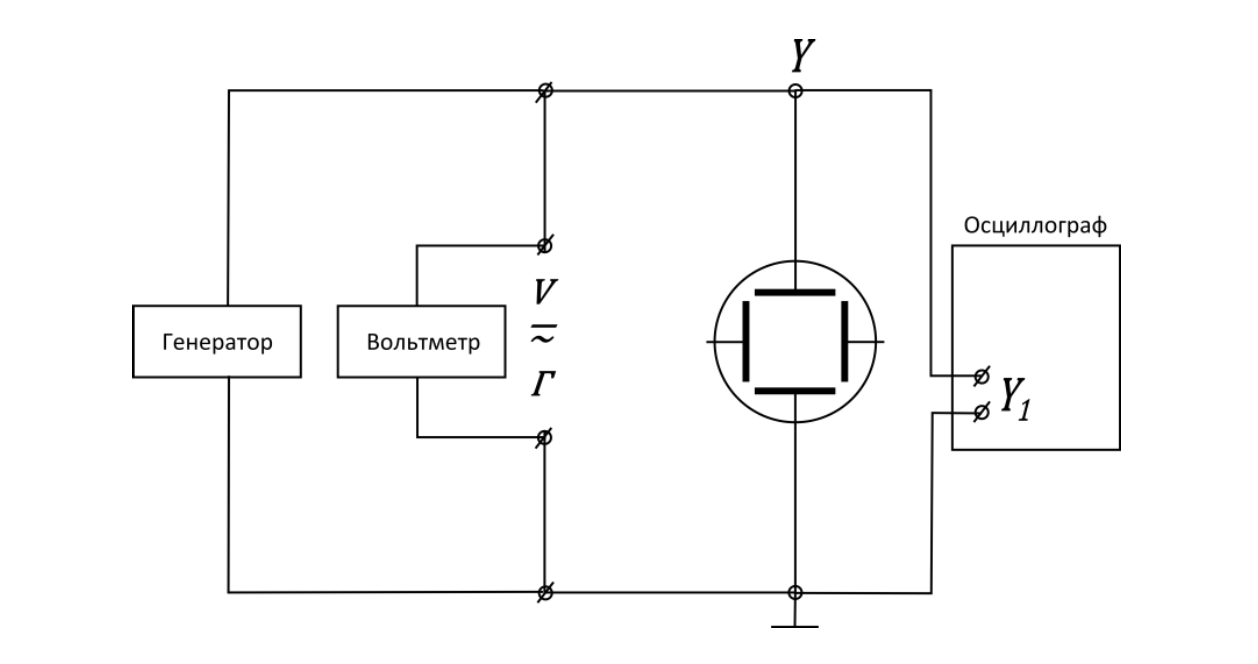
\includegraphics[width=0.8\textwidth]{макс.png}
\caption{Схема электрической цепи для наблюдения исследуемого напряжения и определения максимальной чувствительности осциллографа.}
\end{figure}

\begin{figure}[H]
\centering
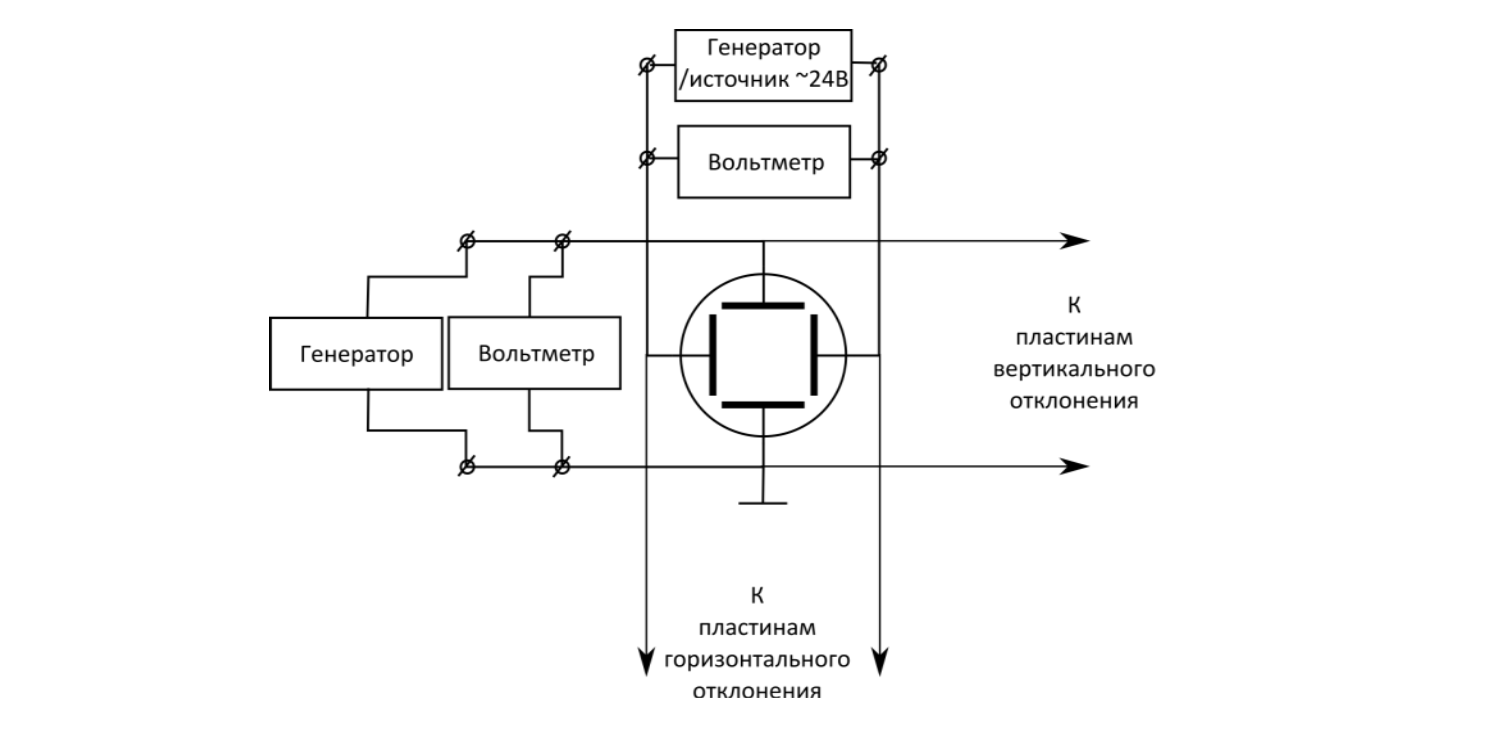
\includegraphics[width=0.8\textwidth]{пластины:лиссажу.png}
\caption{Схема электрической цепи для исследования чувствительности пластин электронно-лучевой трубки и получения фигур Лиссажу.}
\end{figure}

\textbf{Эксперимент проводился в следующей последовательности:}
\begin{enumerate}
\item Ознакомление с работой осциллографа, генератора и вольтметра, подготовка приборов к работе.
\item Сборка схемы с использованием платы №1 для исследования чувствительности пластин.
\item Измерение чувствительности пластины при различных значениях напряжения, подаваемого на пластины вертикального отклонения (ПВО).
\item Измерение чувствительности пластины при различных значениях напряжения, подаваемого на пластины горизонтального отклонения (ПГО).
\item Сборка схемы с использованием платы №2 для вычисления максимальной чувствительности осциллографа.
\item Подключение к пластинам двух синусоидальных напряжений от разных источников для получения фигур Лиссажу.
\item Получение фигур Лиссажу при различных соотношениях частот и определение неизвестной частоты исследуемого напряжения.
\item Запись результатов измерений в таблицы для последующей обработки.
\end{enumerate}
\subsection{Обработка результатов измерений}

По результатам измерений определялась чувствительность пластин вертикального и горизонтального отклонения.

Чувствительность пластин вычислялась по формуле:

\[
S = \frac{L}{2\sqrt{2} \cdot U_{eff}}
\]

где \( L \) — длина светящейся полосы на экране (в мм), \( U_{eff} \) — эффективное значение напряжения, измеренное вольтметром (в В).

Для каждой пары пластин рассчитывались значения чувствительности при разных напряжениях. По полученным данным строились графики зависимости чувствительности ПГО и ПВО от эффективного напряжения.

\begin{figure}[H]
\centering
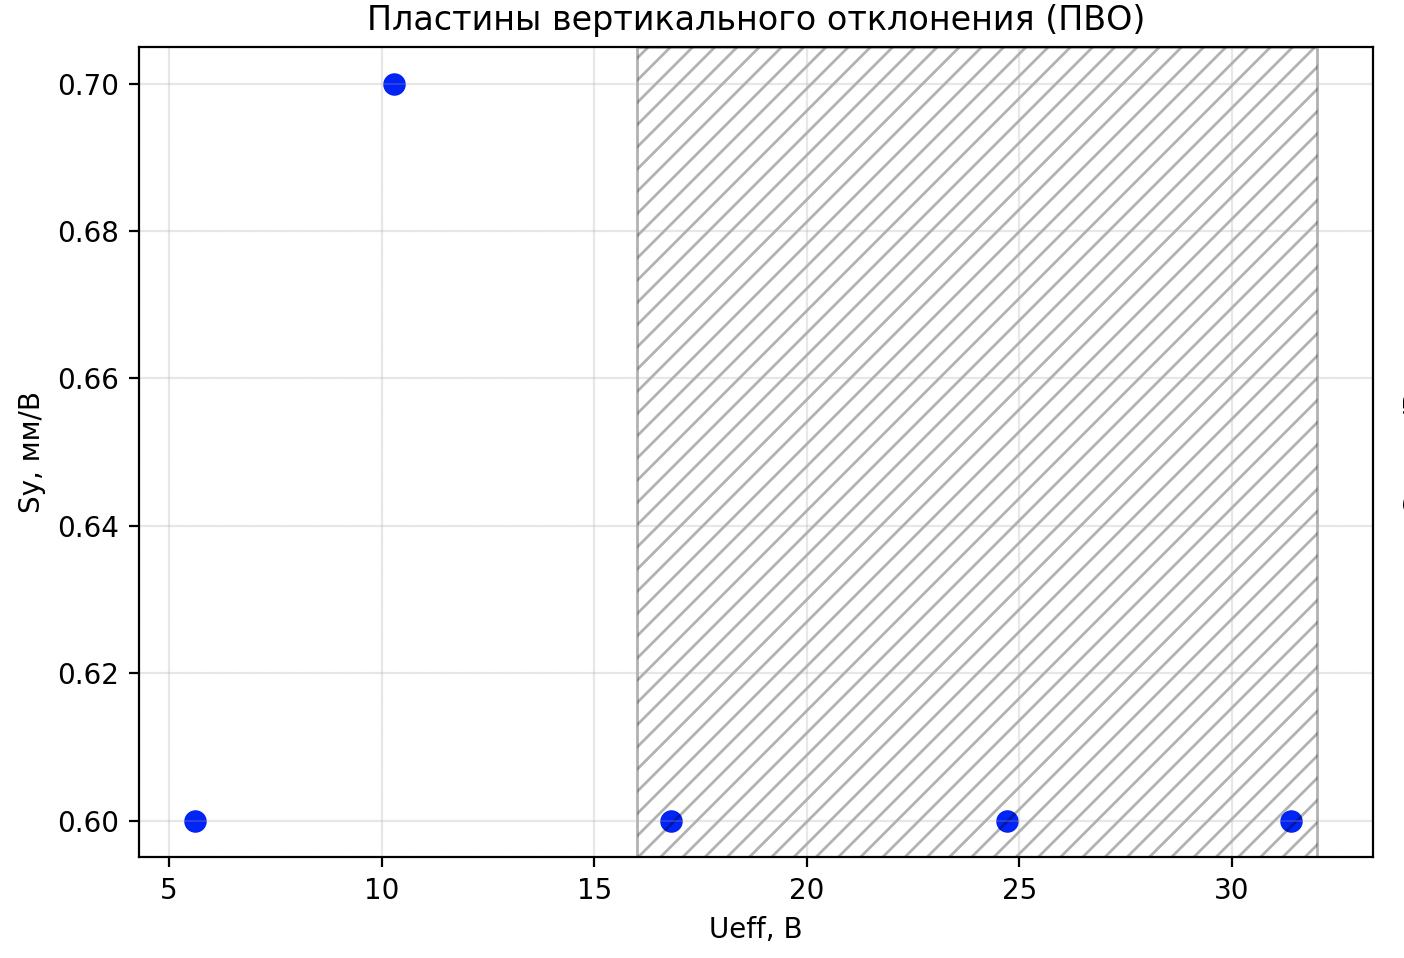
\includegraphics[width=0.8\textwidth]{пво.png}
\caption{График зависимости \(S_y=f(U_\text{eff})\)}
\end{figure}

\begin{figure}[H]
\centering
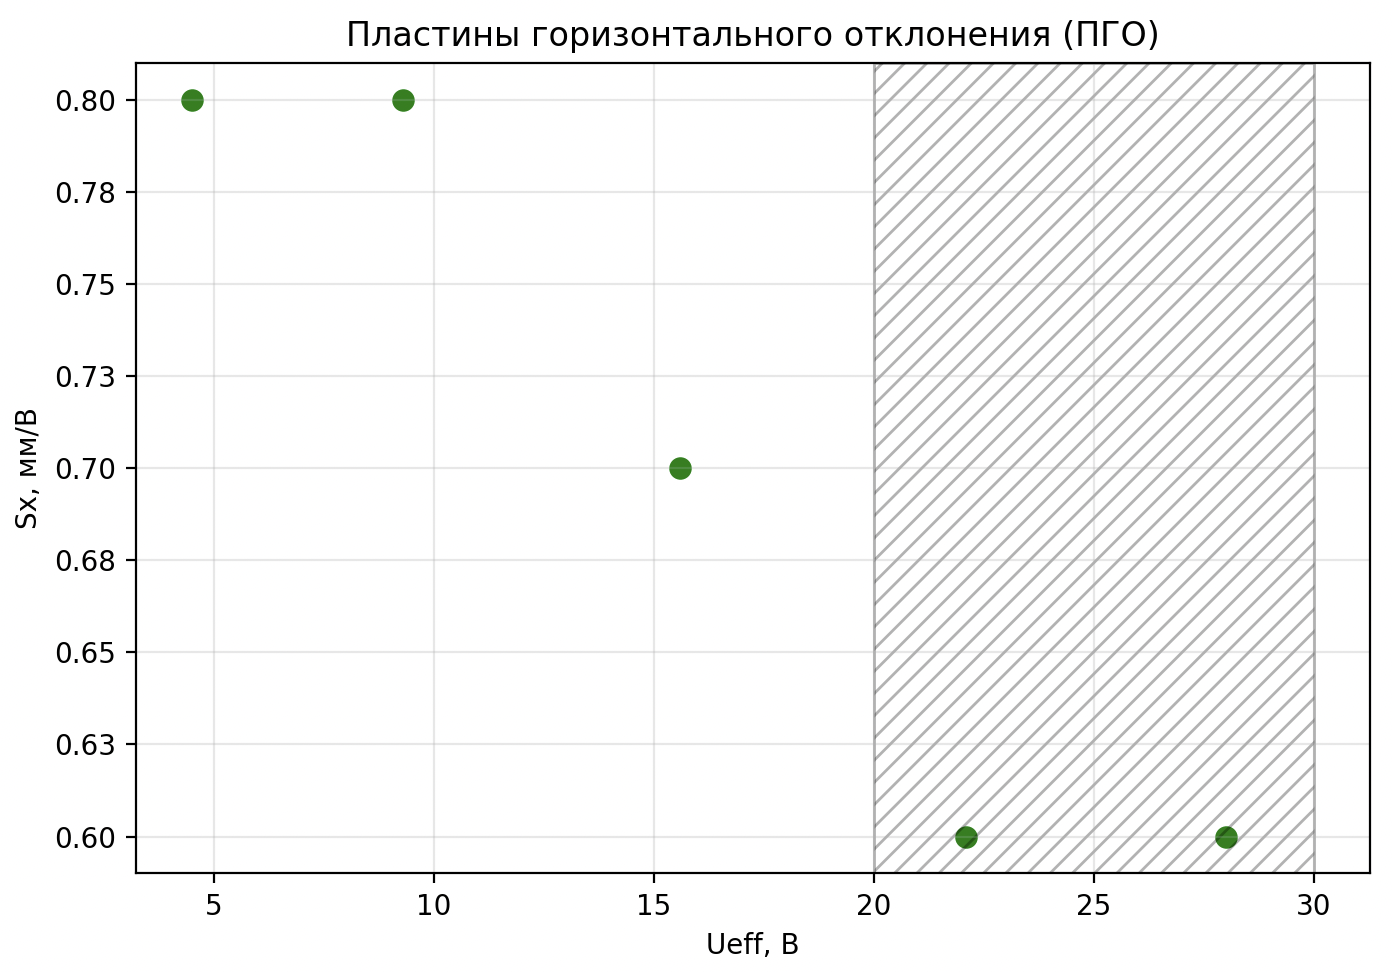
\includegraphics[width=0.8\textwidth]{пго.png}
\caption{График зависимости \(S_x=f(U_\text{eff})\)}
\end{figure}

На графиках \( S_y = f(U_{\text{eff}}) \) и \( S_x = f(U_{\text{eff}}) \) (Рис. 3 и Рис. 4) были выделены участки, на которых чувствительность пластин слабо зависила от эффективного напряжения. Также эти участки называются областью постоянной чувствительности.

Для пластин вертикального отклонения (ПВО) в область постоянной чувствительности попали точки, соответствующие напряжению от 16.8 В до 31.4 В. Для пластин горизонтального отклонения (ПГО) область постоянной чувствительности соответствует диапазону напряжений от 22.1 В до 28.0 В.

\subsubsection{Расчет среднего значения чувствительности и погрешности для ПВО}

Значения чувствительности на выделенном участке для ПВО:
\[
S_{1} = 0.6 \ \text{мм/В}, \quad S_{2} = 0.6 \ \text{мм/В}, \quad S_{3} = 0.6 \ \text{мм/В}
\]

Среднее значение чувствительности вычисляется по формуле:
\[
\bar{S}_y = \frac{1}{n} \sum_{i=1}^{n} S_{i}
\]

Подставляя значения:
\[
\bar{S}_y = \frac{0.6 + 0.6 + 0.6}{3} = 0.6 \ \text{мм/В}
\]

Для оценки погрешности результатов прямых измерений используем среднеквадратичное отклонение от среднего:
\[
\sigma_y = \sqrt{\frac{\sum_{i=1}^{n} (S_{i} - \bar{S}_y)^2}{n-1}}
\]

Вычисляем отклонения от среднего:
\[
S_{1} - \bar{S}_y = 0.6 - 0.6 = 0
\]
\[
S_{2} - \bar{S}_y = 0.6 - 0.6 = 0
\]
\[
S_{3} - \bar{S}_y = 0.6 - 0.6 = 0
\]

Сумма квадратов отклонений:
\[
\sum_{i=1}^{3} (S_{i} - \bar{S}_y)^2 = 0^2 + 0^2 + 0^2 = 0
\]

Тогда среднеквадратичное отклонение:
\[
\sigma_y = \sqrt{\frac{0}{3-1}} = 0.0 \ \text{мм/В}
\]

Таким образом, чувствительность пластин вертикального отклонения в области постоянной чувствительности составляет:
\[
S_y = (0.6 \pm 0.0) \ \text{мм/В}
\]

\subsubsection{Расчет среднего значения чувствительности и погрешности для ПГО}

Значения чувствительности на выделенном участке для ПГО:
\[
S_{1} = 0.6 \ \text{мм/В}, \quad S_{2} = 0.6 \ \text{мм/В}
\]

Среднее значение чувствительности:
\[
\bar{S}_x = \frac{0.6 + 0.6}{2} = 0.6 \ \text{мм/В}
\]

Отклонения от среднего:
\[
S_{1} - \bar{S}_x = 0.6 - 0.6 = 0
\]
\[
S_{2} - \bar{S}_x = 0.6 - 0.6 = 0
\]

Сумма квадратов отклонений:
\[
\sum_{i=1}^{2} (S_{i} - \bar{S}_x)^2 = 0
\]

Среднеквадратичное отклонение:
\[
\sigma_x = \sqrt{\frac{0}{2-1}} = 0.0 \ \text{мм/В}
\]

Таким образом, чувствительность пластин горизонтального отклонения в области постоянной чувствительности составляет:
\[
S_x = (0.6 \pm 0.0) \ \text{мм/В}
\]

Полученные значения погрешности равны нулю, что соответствует тому, что на выделенных участках все измеренные значения чувствительности совпадают (0.6 мм/В). Это говорит о постоянстве чувствительности пластин в данных диапазонах напряжений. 

\subsubsection{Расчёт максимального коэффициента усиления осциллографического усилителя}
Коэффициент усиления усилителя вертикального отклонения рассчитывается по формуле:

\[
K = \frac{(S'_y)_m}{S_y}
\]

где \((S'_y)_m\) — максимальная чувствительность осциллографа по входу Y, \(S_y\) — чувствительность пластин вертикального отклонения.

Чувствительность пластин вертикального отклонения в области постоянной чувствительности составляет \(S_y = 0.600\) мм/В. Максимальная чувствительность осциллографа, достигнутая в эксперименте (при L = 20 мм, \(U_{eff}\) = 0.020 В), равна \((S'_y)_m = 353.553\) мм/В.

Подставляя значения:

\[
K = \frac{353.553}{0.600} = 589.255
\] 

Таким образом, коэффициент усиления усилителя вертикального отклонения составляет:

\[
K = 589.255
\]
Следовательно, усилитель вертикального отклонения увеличивает чувствительность осциллографа в 589.255 раза, что позволяет наблюдать сигналы малой амплитуды.
\subsubsection{Определение частоты генератора по фигурам Лиссажу}
Определение неизвестной частоты по фигурам Лиссажу производилось методом касательных. Для каждой полученной фигуры подсчитывалось число касаний с горизонтальной \( n_x \) и вертикальной \( n_y \) сторонами ограничивающего прямоугольника. Неизвестная частота вычислялась по формуле:

\[
f_x = f_y \cdot \frac{n_y}{n_x}
\]

где \( f_y \) — известная частота генератора.

Во всех случаях было получено значение \(f_x = 50\) Гц. 
Среднее значение частоты вычисляется по формуле:

\[
\bar{f}_x = \frac{1}{n} \sum_{i=1}^{n} f_{i}
\]

Подставляя значения:

\[
\bar{f}_x = \frac{50 + 50 + 50 + 50}{4} = 50.000 \ \text{Гц}
\]

Для оценки погрешности результата используется среднеквадратичное отклонение от среднего:

\[
\sigma = \sqrt{\frac{\sum_{i=1}^{n} (f_{i} - \bar{f}_x)^2}{n-1}}
\]

Так как все значения равны среднему, отклонения равны нулю:

\[
\sum (f_{i} - \bar{f}_x)^2 = 0
\]

Следовательно:

\[
\sigma = \sqrt{\frac{0}{4-1}} = 0.000 \ \text{Гц}
\]

Таким образом, результат измерения частоты генератора:

\[
f_x = (50.000 \pm 0.000) \ \text{Гц}
\]

Полученная нулевая погрешность объясняется тем, что все измерения дали одинаковое значение частоты.

\section{Вывод}
В ходе исследования были исследованы основные характеристики электронного осциллографа.

\textbf{Чувствительность пластин вертикального и горизонтального отклонения.} 
    Экспериментально определены значения чувствительности при непосредственном подключении генератора к отклоняющим пластинам. Для пластин вертикального отклонения (ПВО) средняя чувствительность составила \(S_y = 0.6 \pm 0.0\) мм/В, для пластин горизонтального отклонения (ПГО) — \(S_x = 0.6 \pm 0.0\) мм/В. 
    
    Одинаковые значения чувствительности в областях постоянной чувствительности можно объяснить тем что в условиях прямого подключения обе пары пластин находились в одинаковых условиях поскольку являются частью одной электронно-лучевой трубки с одинаковыми геометрическими параметрами и режимом питания. Нулевая погрешность может быть связана с малым количеством измерений, однако в целом говорит об их стабильности.

 \textbf{Коэффициент усиления усилителя вертикального отклонения.} 
    Рассчитанный коэффициент усиления 
    \[
    K = \frac{S'_y}{S_y} = \frac{353.553}{0.600} = 589.255
    \]
    показывает, что усилитель увеличивает отклонение луча в 589,255 раз. Благодаря чему осциллограф способен регистрировать сигналы малой амплитуды, которые без усиления оставались бы незаметными на экране.

    \textbf{Определение частоты методом фигур Лиссажу.} 
    При известной частоте \(f_y\), по фигурам Лиссажу для соотношений 1:1, 2:1, 3:1 и 1:2 была определена частота генератора \(f_x\). Во всех случаях получено значение \(f_x = 50.000 \pm 0.000\) Гц. Это подтверждает высокую точность и надёжность метода фигур Лиссажу для сравнения и измерения частот.

Таким образом, все поставленные задачи и цель работы выполнены. Полученные результаты позволяют лучше понять принципы работы осциллографа.
\clearpage
\appendix


\end{document}
